% !TeX root = main.tex

\setlength{\abovedisplayskip}{7pt}
\setlength{\belowdisplayskip}{7pt}
\setlength{\abovedisplayshortskip}{4pt}
\setlength{\belowdisplayshortskip}{4pt}

% Рисунок и подпись располагаются рядом с соответствующим текстом.
\makeatletter
\newenvironment{reportfigure}{%
  \par\addvspace{8pt}\noindent
  \begin{minipage}{\textwidth}
    \def\@captype{figure}%
    \centering
}{%
  \end{minipage}\par\vspace{4pt}
}
\makeatother

\tableofcontents
\newpage

\section{Цель работы}

Синтезировать апериодический регулятор, регулятор Далина и регулятор
с заданным расположением полюсов замкнутой системы. Исследовать
переходные процессы и точность воспроизведения задающих воздействий.

\section{Исходные данные}

Для варианта 3 непрерывный объект задан передаточной функцией
\begin{equation}
  G(s)=\frac{e^{-as}}{1+bs}
      =\frac{e^{-2s}}{1+4s},
  \qquad a=2\,\text{с},\qquad b=4\,\text{с}
  \label{eq:continuous-plant}
\end{equation}
При синтезе апериодического регулятора и регулятора Далина принимаем
$T=1\,\text{с}$ согласно заданию. В задаче с заданным расположением
полюсов используем $T=0{,}2\,\text{с}$ согласно варианту.

Обозначим через $G_{\text{д}}(z)$ передаточную функцию объекта
с экстраполятором нулевого порядка, а через $\Phi(z)$ обозначим
желаемую передаточную функцию замкнутой системы.
При единичной отрицательной обратной связи имеем
\begin{equation}
  \Phi(z)=\frac{Y(z)}{R(z)},
  \qquad D(z)=\frac{1}{G_{\text{д}}(z)}\frac{\Phi(z)}{1-\Phi(z)}
  \label{eq:controller-formula}
\end{equation}

\section{Апериодический регулятор}

\subsection{Дискретная модель объекта}

Запаздывание составляет два периода дискретизации. Введём обозначения
\begin{equation}
  d=\frac{a}{T}=2,
  \qquad p=e^{-T/b}=e^{-0{,}25}\approx0{,}77880078,
  \qquad 1-p\approx0{,}22119922
  \label{eq:zoh-coefficients}
\end{equation}
Точная дискретизация объекта с удержанием управления даёт
\begin{equation}
  G_{\text{д}}(z)
  =\frac{(1-p)z^{-(d+1)}}{1-pz^{-1}}
  \approx\frac{0{,}22119922z^{-3}}{1-0{,}77880078z^{-1}}
  \label{eq:zoh-plant}
\end{equation}
Дополнительный сдвиг на один отсчёт обусловлен строго правильной
передаточной функцией апериодического звена.

\subsection{Синтез регулятора}

Для установления выхода за конечное число отсчётов выбираем
\begin{equation}
  \Phi(z)=z^{-N}
  \label{eq:deadbeat-reference}
\end{equation}
После подстановки в~\eqref{eq:controller-formula} получаем
\begin{equation}
  D(z)=\frac{1-pz^{-1}}{1-p}
       \frac{z^{3-N}}{1-z^{-N}}
  \label{eq:deadbeat-family}
\end{equation}
Физическая реализуемость требует отсутствия опережения,
поэтому минимально допустимым является значение $N=3$ отсчёта.
Для этого значения регулятор имеет вид
\begin{equation}
  D(z)=\frac{1-pz^{-1}}{(1-p)(1-z^{-3})}
      =\frac{z^3-pz^2}{(1-p)(z^3-1)}
  \label{eq:deadbeat-controller}
\end{equation}
Численно получаем
\begin{equation}
  D(z)\approx\frac{4{,}52081166z^3-3{,}52081166z^2}{z^3-1}
  \label{eq:deadbeat-controller-numeric}
\end{equation}
Желаемая передаточная функция замкнутой системы равна
\begin{equation}
  \Phi(z)=z^{-3}
  \label{eq:deadbeat-closed-loop}
\end{equation}

\subsection{Моделирование}

Моделирование проводилось в течение $7\,\text{с}$ при нулевых начальных
состояниях объекта и регулятора. В начальный момент подавалось единичное
ступенчатое задание. Непрерывный объект реализован как последовательное
соединение звена $1/(4s+1)$ и задержки на $2\,\text{с}$;
управление удерживается между отсчётами, а выход поступает в обратную
связь через выборку с периодом $T=1\,\text{с}$ согласно расчёту.

На рисунке~\ref{fig:deadbeat} сплошной линией показан непрерывный выход,
маркерами отмечены его значения в моменты выборки. Снизу приведено
управляющее воздействие.

\begin{reportfigure}
  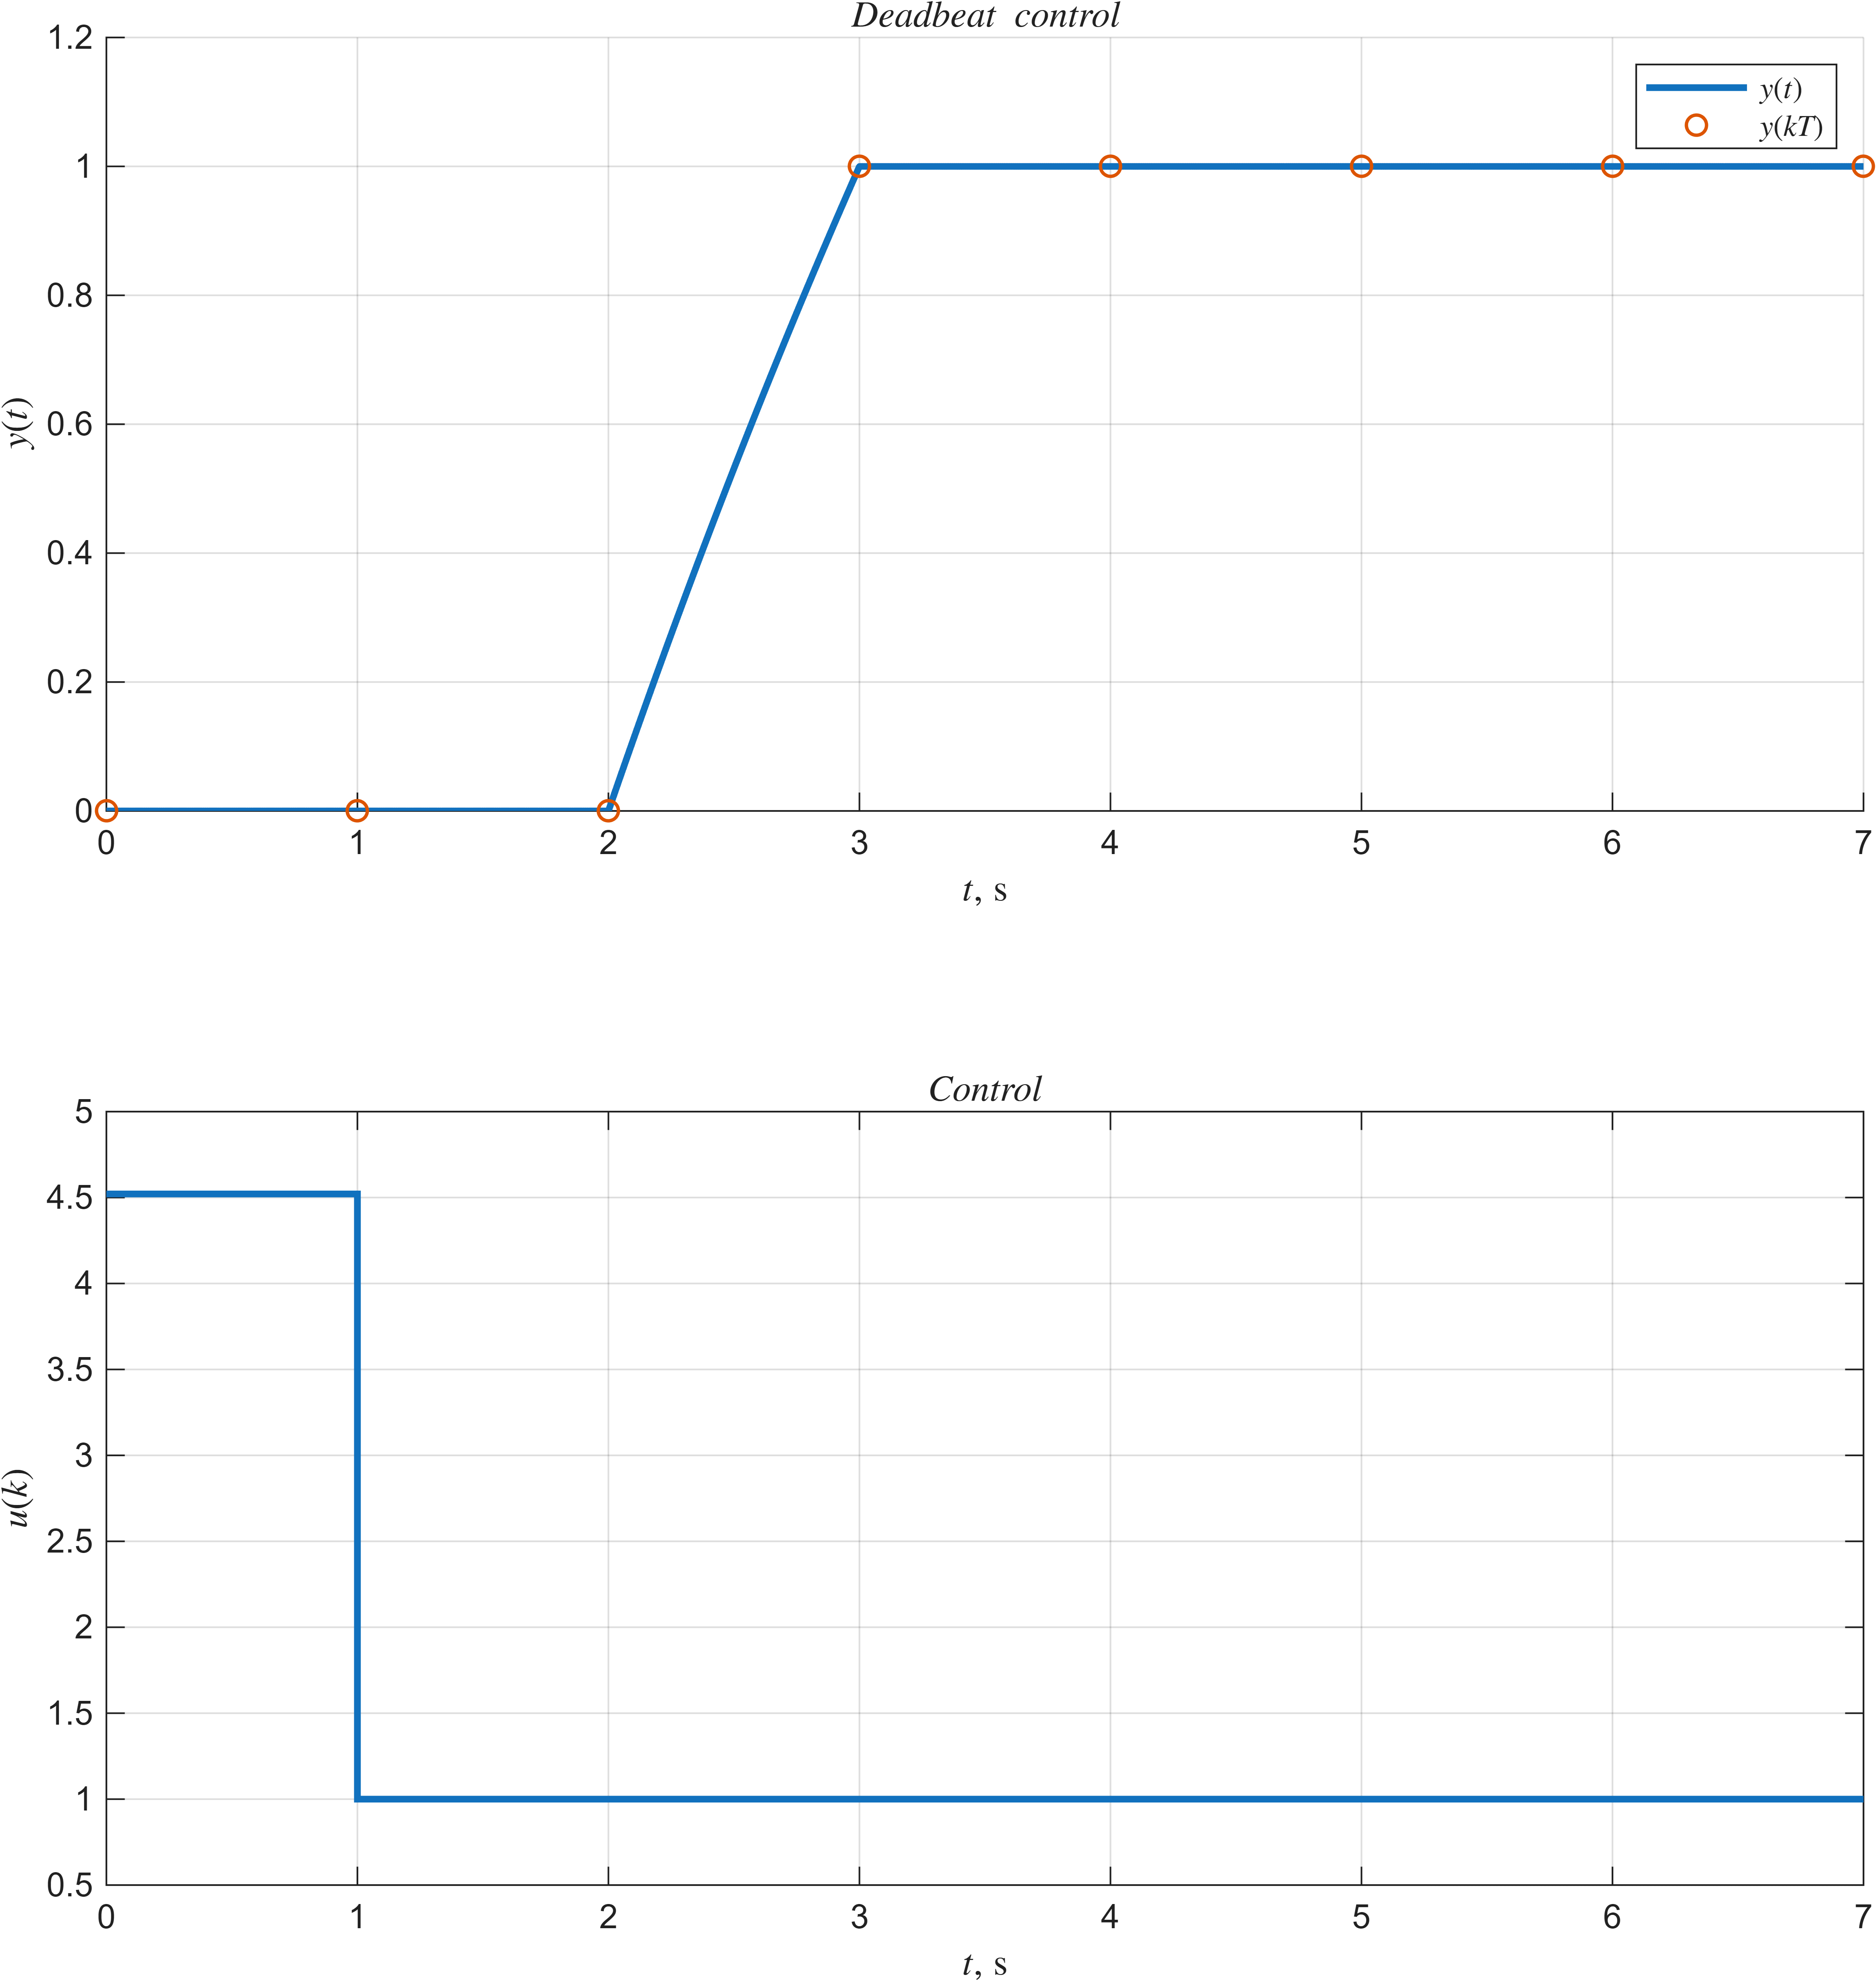
\includegraphics[width=\textwidth,height=0.7\textheight,keepaspectratio]{task1_deadbeat.png}
  \caption{Выход системы и управление с апериодическим регулятором}
  \label{fig:deadbeat}
\end{reportfigure}

В течение первых двух секунд выход остаётся нулевым из-за запаздывания.
Затем он монотонно возрастает и в момент $t=3\,\text{с}$ достигает
единицы. Начиная с третьего отсчёта выход сохраняет заданное значение
с точностью численного расчёта. Это соответствует полученной передаточной
функции $\Phi(z)=z^{-3}$ замкнутой системы. Между отсчётами выход
изменяется непрерывно, без перерегулирования на рассматриваемом интервале.

На первом интервале дискретизации управление составляет примерно
$4{,}52$, после чего уменьшается до единицы и остаётся постоянным.
Таким образом, быстрое установление выхода обеспечивается повышенным
начальным управляющим воздействием.

\section{Регулятор Далина}

\subsection{Желаемая передаточная функция}

Для того же объекта~\eqref{eq:zoh-plant} задаём экспоненциальную
реакцию с запаздыванием. Постоянную времени желаемого процесса
принимаем равной постоянной времени объекта:
\begin{equation}
  q=b=4\,\text{с},
  \qquad \lambda=e^{-T/q}=e^{-0{,}25}=p\approx0{,}77880078
  \label{eq:dahlin-coefficient}
\end{equation}
Желаемая передаточная функция имеет вид
\begin{equation}
  \Phi(z)=\frac{(1-\lambda)z^{-3}}{1-\lambda z^{-1}}
  \label{eq:dahlin-reference}
\end{equation}

\subsection{Расчёт регулятора}

Из~\eqref{eq:controller-formula} получаем
\begin{equation}
  D(z)=\frac{1-\lambda}{1-p}
       \frac{1-pz^{-1}}{1-\lambda z^{-1}-(1-\lambda)z^{-3}}
  \label{eq:dahlin-controller}
\end{equation}
При выбранном значении $q$ множитель $(1-\lambda)/(1-p)$ равен единице.
В положительных степенях переменной $z$ получаем
\begin{equation}
  D(z)=\frac{z^3-pz^2}{z^3-pz^2-(1-p)}
    \approx\frac{z^3-0{,}77880078z^2}
       {z^3-0{,}77880078z^2-0{,}22119922}
  \label{eq:dahlin-controller-numeric}
\end{equation}
Порядки числителя и знаменателя равны, поэтому полученный регулятор
физически реализуем.

\subsection{Моделирование}

Начальные состояния, единичное ступенчатое задание и реализация объекта
сохраняются такими же, как в предыдущем опыте. Интервал моделирования
увеличен до $40\,\text{с}$ для наблюдения более медленного переходного
процесса. Результаты приведены на рисунке~\ref{fig:dahlin}.

\begin{reportfigure}
  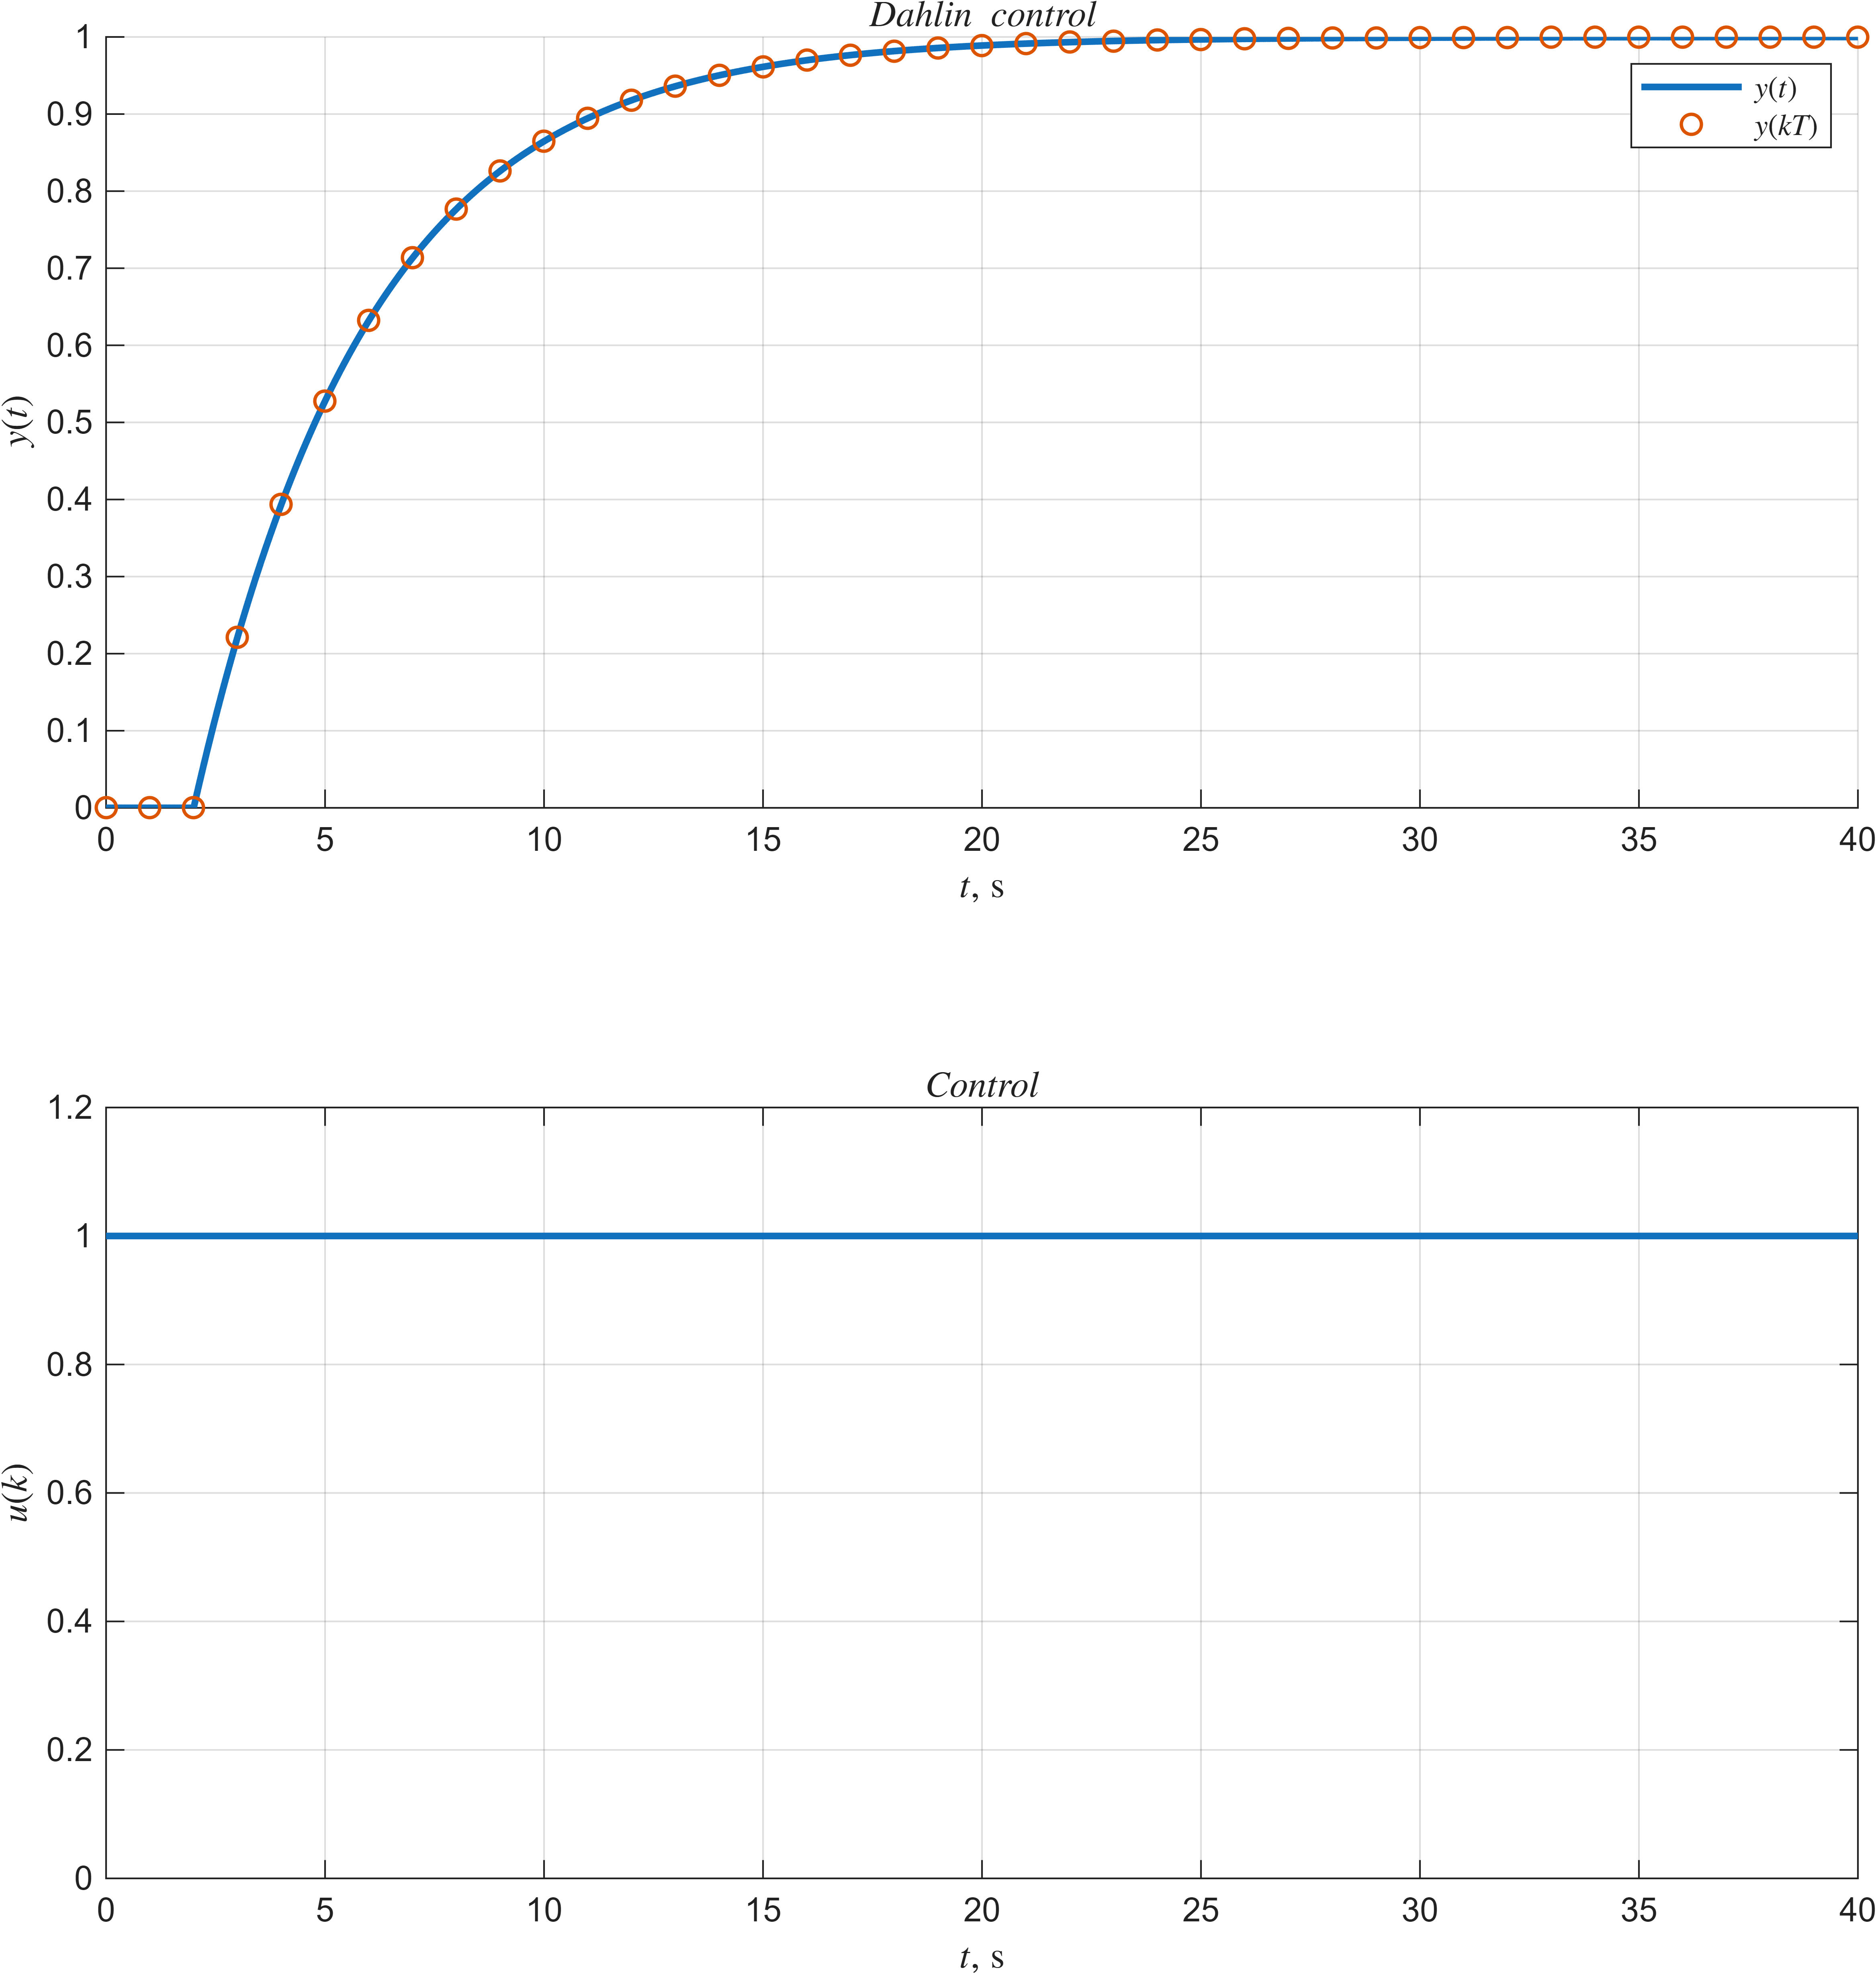
\includegraphics[width=\textwidth,height=0.7\textheight,keepaspectratio]{task2_dahlin.png}
  \caption{Выход системы и управление с регулятором Далина}
  \label{fig:dahlin}
\end{reportfigure}

После двухсекундного запаздывания выход монотонно приближается к единице.
Перерегулирование и колебания между отсчётами на графике отсутствуют.
К двадцатой секунде выход уже близок к заданному значению,
но установление происходит заметно медленнее, чем с апериодическим
регулятором.

При выбранном значении $q=b$ управление равно единице на всём интервале.
По сравнению с апериодическим регулятором начальное управляющее воздействие
уменьшается примерно с $4{,}52$ до единицы. Более плавный переходный
процесс сопровождается снижением быстродействия.

\section{Регулятор с заданным расположением полюсов}

\subsection{Объект и требования к замкнутой системе}

В этой части дискретный объект задан непосредственно:
\begin{equation}
  G_{\text{д}}(z)=\frac{0{,}03(z+0{,}75)}{z^2-1{,}5z+0{,}5}
  \label{eq:pole-placement-plant}
\end{equation}
Параметры варианта 3 равны
\begin{equation}
  T=0{,}2\,\text{с},\qquad \zeta=0{,}7,
  \qquad \omega_d=5\,\text{рад/с},\qquad K_v=0{,}25
  \label{eq:pole-placement-data}
\end{equation}
Здесь согласно заданию $K_v$ обозначает требуемую установившуюся
ошибку при $r(k)=kT$ для единичного линейно нарастающего воздействия.
Ошибка при единичном ступенчатом воздействии должна быть нулевой.

\subsection{Желаемые полюса}

Собственная частота и желаемые полюса определяются выражениями
\begin{equation}
  \omega_n=\frac{\omega_d}{\sqrt{1-\zeta^2}}
       \approx7{,}00140042\,\text{рад/с},
  \qquad
  z_{1,2}=e^{-\zeta\omega_nT}
        \bigl(\cos(\omega_dT)\pm j\sin(\omega_dT)\bigr)
  \label{eq:desired-poles}
\end{equation}
После подстановки численных параметров получаем
\begin{equation}
  z_{1,2}\approx0{,}20274170\pm j\,0{,}31575149
  \label{eq:desired-poles-numeric}
\end{equation}
Соответствующий полином равен
\begin{equation}
  P(z)=(z-z_1)(z-z_2)
       \approx z^2-0{,}40548340z+0{,}14080320
  \label{eq:desired-polynomial}
\end{equation}
Желаемую передаточную функцию выбираем в виде
\begin{equation}
  \Phi(z)=\frac{b_1z+b_2}{P(z)}
  \label{eq:pole-placement-reference}
\end{equation}

\subsection{Расчёт числителя по условиям точности}

Для единичного ступенчатого воздействия условие нулевой
установившейся ошибки даёт
\begin{equation}
  \Phi(1)=1,
  \qquad b_1+b_2=P(1)\approx0{,}73531980
  \label{eq:step-accuracy}
\end{equation}
Для линейного воздействия $r(k)=kT$ имеем
\begin{equation}
  R(z)=\frac{Tz}{(z-1)^2},
  \qquad E(z)=R(z)\bigl(1-\Phi(z)\bigr)
  \label{eq:ramp-error}
\end{equation}
По теореме о конечном значении получаем второе условие:
\begin{equation}
  e_{\text{уст}}=-T\Phi'(1)=K_v,
  \qquad \Phi'(1)=-\frac{0{,}25}{0{,}2}=-1{,}25
  \label{eq:ramp-accuracy}
\end{equation}
Подстановка~\eqref{eq:pole-placement-reference} даёт
\begin{equation}
  \Phi'(1)
    =\frac{b_1-P'(1)}{P(1)}=-1{,}25
  \label{eq:numerator-equation}
\end{equation}
Решая совместно~\eqref{eq:step-accuracy} и~\eqref{eq:numerator-equation},
получаем
\begin{equation}
  b_1\approx0{,}67536685,
  \qquad b_2\approx0{,}05995295
  \label{eq:numerator-coefficients}
\end{equation}
Таким образом,
\begin{equation}
  \Phi(z)\approx
  \frac{0{,}67536685z+0{,}05995295}
       {z^2-0{,}40548340z+0{,}14080320}
  \label{eq:pole-placement-reference-numeric}
\end{equation}

\subsection{Передаточная функция регулятора}

Подставляем желаемую функцию в~\eqref{eq:controller-formula}:
\begin{equation}
  D(z)=\frac{(z^2-1{,}5z+0{,}5)(b_1z+b_2)}
  {0{,}03(z+0{,}75)\bigl(P(z)-b_1z-b_2\bigr)}
  \label{eq:pole-placement-controller}
\end{equation}
Условие~\eqref{eq:step-accuracy} позволяет выделить общий множитель:
\begin{equation}
  P(z)-b_1z-b_2=(z-1)(z-c),
  \qquad c=1-\frac{K_v}{T}P(1)\approx0{,}08085025
  \label{eq:controller-factorization}
\end{equation}
Учитывая $z^2-1{,}5z+0{,}5=(z-1)(z-0{,}5)$,
после сокращения получаем
\begin{equation}
  D(z)=\frac{(z-0{,}5)(b_1z+b_2)}
             {0{,}03(z+0{,}75)(z-c)}
  \label{eq:pole-placement-controller-reduced}
\end{equation}
Численная передаточная функция регулятора имеет вид
\begin{equation}
  D(z)\approx
  \frac{22{,}51222837z^2-9{,}25768253z-0{,}99921583}
       {z^2+0{,}66914975z-0{,}06063769}
  \label{eq:pole-placement-controller-numeric}
\end{equation}
Полученный регулятор физически реализуем, поскольку порядки
числителя и знаменателя совпадают.

\subsection{Моделирование}

Моделирование выполнялось в течение $4\,\text{с}$ при нулевых начальных
состояниях объекта и регулятора. В отдельных контурах подавались
единичное ступенчатое задание и линейное задание $r(k)=kT$ с единичной
скоростью роста. Во всех дискретных звеньях используется период
$T=0{,}2\,\text{с}$ согласно варианту.

На рисунке~\ref{fig:pole-placement} слева показаны выход и задание,
справа приведены ошибки слежения. Верхние графики соответствуют
ступенчатому воздействию, нижние соответствуют линейному.

\begin{reportfigure}
  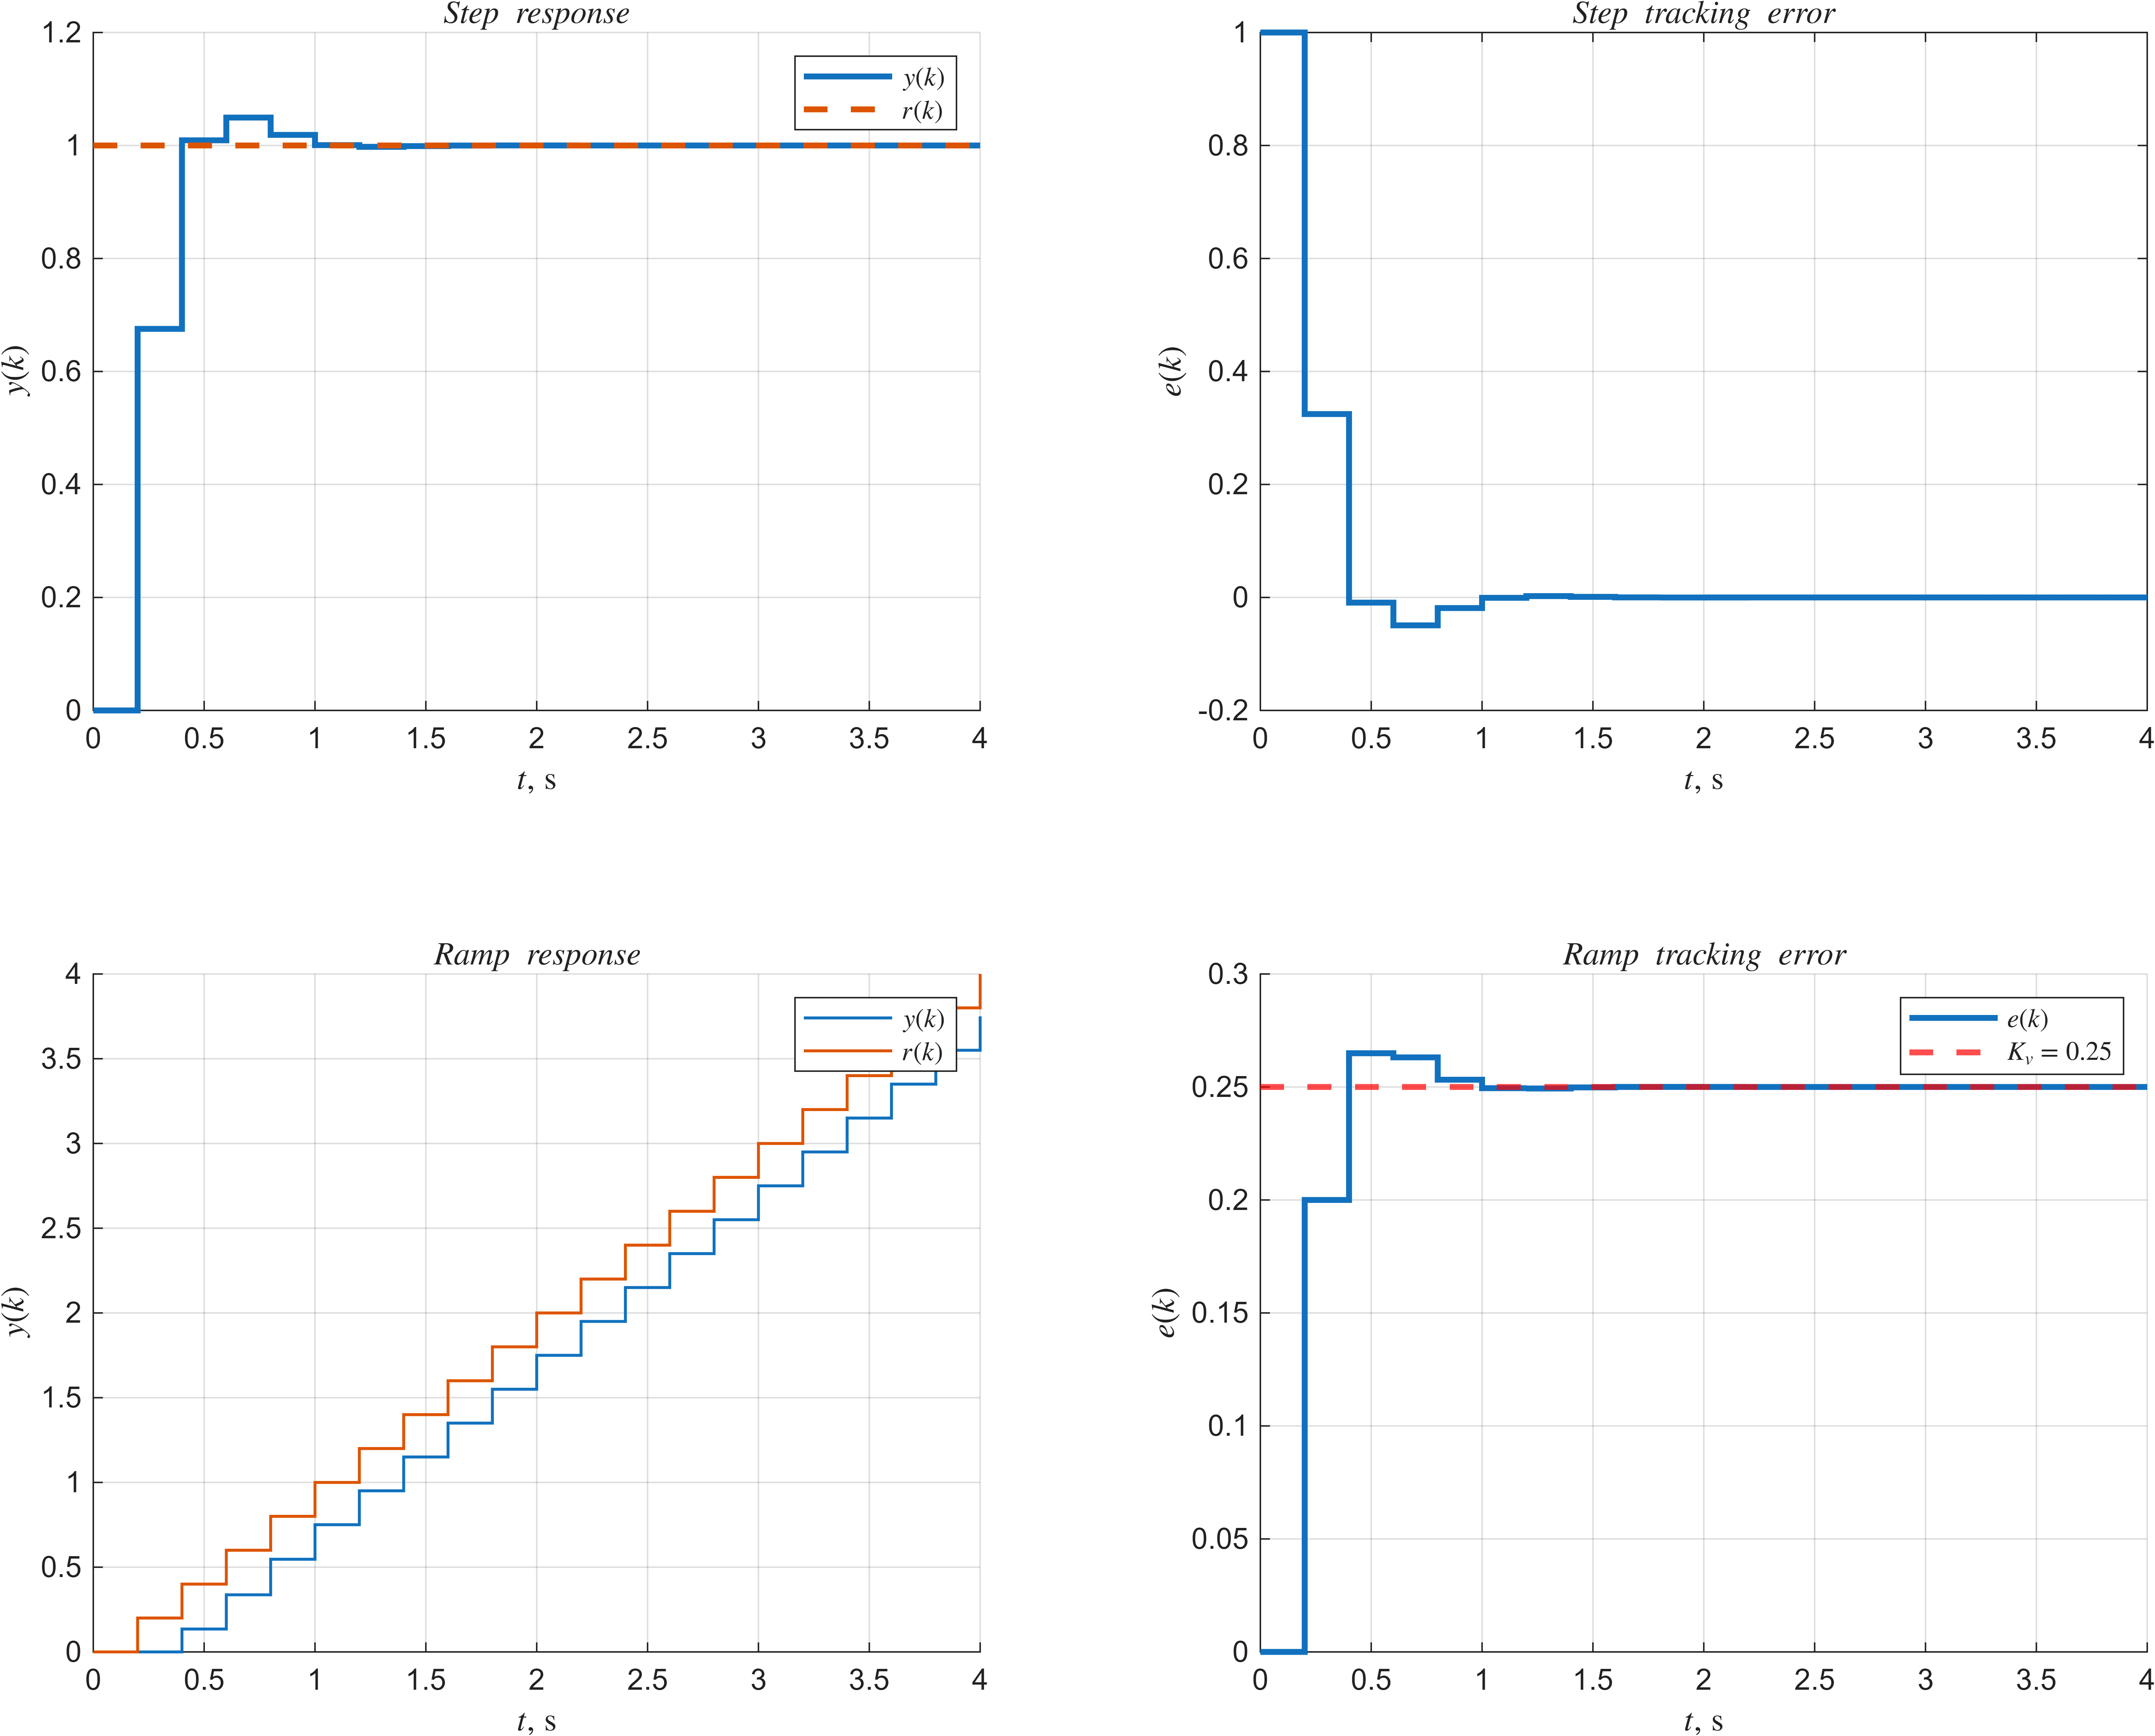
\includegraphics[width=\textwidth,keepaspectratio]{task3_poles.png}
  \caption{Выход и ошибка системы с заданными полюсами при ступенчатом и линейном воздействиях}
  \label{fig:pole-placement}
\end{reportfigure}

При ступенчатом воздействии выход имеет затухающий колебательный
переходный процесс. Максимум составляет примерно $1{,}049$ в момент
$t=0{,}6\,\text{с}$, что соответствует перерегулированию около пяти
процентов. После переходного процесса выход стремится к единице,
а ошибка слежения стремится к нулю. Это согласуется с условием
нулевой установившейся ошибки при постоянном задании.

При линейном воздействии выход после переходного процесса растёт
с той же скоростью, что и задание, сохраняя постоянное отставание.
Ошибка сначала достигает примерно $0{,}265$, затем стремится
к требуемому значению $K_v=0{,}25$ и к концу интервала совпадает
с ним в масштабе рисунка. Таким образом, оба требования
к установившимся ошибкам выполняются.

\clearpage
\section{Выводы}

Апериодический регулятор обеспечивает достижение единичного задания
за три периода дискретизации. После установления выход сохраняет
заданное значение с точностью численного расчёта. Быстродействие
достигается за счёт начального управления примерно $4{,}52$ на первом
интервале дискретизации.

Регулятор Далина при выбранной постоянной времени обеспечивает
монотонный переходный процесс без перерегулирования. Управление
остаётся единичным, однако выход приближается к заданию медленнее,
чем в системе с апериодическим регулятором.

Регулятор с заданным расположением полюсов обеспечивает затухающий
колебательный переходный процесс. Установившаяся ошибка при ступенчатом
воздействии равна нулю, а при линейном воздействии стремится к заданному
значению $0{,}25$ согласно требованиям работы.
